\documentclass[]{article}
\usepackage{lmodern}
\usepackage{amssymb,amsmath}
\usepackage{ifxetex,ifluatex}
\usepackage{fixltx2e} % provides \textsubscript
\ifnum 0\ifxetex 1\fi\ifluatex 1\fi=0 % if pdftex
  \usepackage[T1]{fontenc}
  \usepackage[utf8]{inputenc}
\else % if luatex or xelatex
  \ifxetex
    \usepackage{mathspec}
  \else
    \usepackage{fontspec}
  \fi
  \defaultfontfeatures{Ligatures=TeX,Scale=MatchLowercase}
\fi
% use upquote if available, for straight quotes in verbatim environments
\IfFileExists{upquote.sty}{\usepackage{upquote}}{}
% use microtype if available
\IfFileExists{microtype.sty}{%
\usepackage{microtype}
\UseMicrotypeSet[protrusion]{basicmath} % disable protrusion for tt fonts
}{}
\usepackage[margin=1in]{geometry}
\usepackage{hyperref}
\hypersetup{unicode=true,
            pdftitle={Biofouling Tutorial},
            pdfauthor={Dr.~Linda Auker},
            pdfborder={0 0 0},
            breaklinks=true}
\urlstyle{same}  % don't use monospace font for urls
\usepackage{graphicx,grffile}
\makeatletter
\def\maxwidth{\ifdim\Gin@nat@width>\linewidth\linewidth\else\Gin@nat@width\fi}
\def\maxheight{\ifdim\Gin@nat@height>\textheight\textheight\else\Gin@nat@height\fi}
\makeatother
% Scale images if necessary, so that they will not overflow the page
% margins by default, and it is still possible to overwrite the defaults
% using explicit options in \includegraphics[width, height, ...]{}
\setkeys{Gin}{width=\maxwidth,height=\maxheight,keepaspectratio}
\IfFileExists{parskip.sty}{%
\usepackage{parskip}
}{% else
\setlength{\parindent}{0pt}
\setlength{\parskip}{6pt plus 2pt minus 1pt}
}
\setlength{\emergencystretch}{3em}  % prevent overfull lines
\providecommand{\tightlist}{%
  \setlength{\itemsep}{0pt}\setlength{\parskip}{0pt}}
\setcounter{secnumdepth}{0}
% Redefines (sub)paragraphs to behave more like sections
\ifx\paragraph\undefined\else
\let\oldparagraph\paragraph
\renewcommand{\paragraph}[1]{\oldparagraph{#1}\mbox{}}
\fi
\ifx\subparagraph\undefined\else
\let\oldsubparagraph\subparagraph
\renewcommand{\subparagraph}[1]{\oldsubparagraph{#1}\mbox{}}
\fi

%%% Use protect on footnotes to avoid problems with footnotes in titles
\let\rmarkdownfootnote\footnote%
\def\footnote{\protect\rmarkdownfootnote}

%%% Change title format to be more compact
\usepackage{titling}

% Create subtitle command for use in maketitle
\newcommand{\subtitle}[1]{
  \posttitle{
    \begin{center}\large#1\end{center}
    }
}

\setlength{\droptitle}{-2em}

  \title{Biofouling Tutorial}
    \pretitle{\vspace{\droptitle}\centering\huge}
  \posttitle{\par}
    \author{Dr.~Linda Auker}
    \preauthor{\centering\large\emph}
  \postauthor{\par}
      \predate{\centering\large\emph}
  \postdate{\par}
    \date{5/7/2019}


\begin{document}
\maketitle

\subsection{Analysis of Community Settlement
Panels}\label{analysis-of-community-settlement-panels}

This site contains tutorials for photographing, analyzing, and
visualizing data for assessing biofouling on panels.

 Go to Option 1: drawing lines around organisms Go to Option 2: using a
grid to count frequency of organisms

\subsection{Option 1: drawing lines around organisms}\label{Option1}

Pros: More accurate. Cons: Time-consuming, particularly for heavily
settled panels.

\subsection{Photographing panels}\label{photographing-panels}

\begin{enumerate}
\def\labelenumi{\arabic{enumi}.}
\item
  Photograph both sides of each panel clearly. The more light available
  and the closest you can get to the panel without cropping it out will
  make it easier to analyze. Use the highest resolution on your
  smartphone or digital camera.
\item
  Send the labeled photos to \_\_\_\_\_\_\_\_\_\_\_\_\_\_\_ (or add to a
  dropbox?). Suggested labeling includes depth\_side\_replicate. So a
  shallow panel front might be Shallow\_front\_1, and the other side of
  the panel is Shallow\_back\_1.
\end{enumerate}

\subsection{Analyzing panel photographs in
ImageJ}\label{analyzing-panel-photographs-in-imagej}

\begin{enumerate}
\def\labelenumi{\arabic{enumi}.}
\item
  Download ImageJ, a free open-source image analysis software available
  from NIH, at \url{https://imagej.nih.gov/ij/download.html}.
\item
  Open the program. Go to File \textgreater{} Open and find your
  photograph in the directory. Once you open your photograph, zoom in or
  out as needed to ensure the entire panel is visible on your screen and
  you are able to see the organisms clearly.
\item
  Set the scale of your image. First, choose the ``Straight Line'' shape
  and draw a line along one edge of your panel.
\end{enumerate}

\begin{figure}
\centering
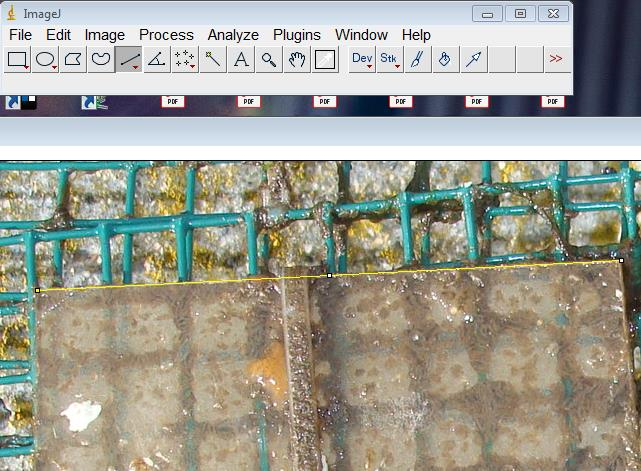
\includegraphics{/images/Figure1.jpg}
\caption{Figure 1}
\end{figure}

Next, go to Analyze \textgreater{} Set Scale\ldots{} . In the dialog
box, the program gives you the distance in pixels of the line you have
drawn. In ``Known distance'' enter the length of the panel (10) and in
``Unit of length'' enter the units used (cm). Click ok.

\begin{enumerate}
\def\labelenumi{\arabic{enumi}.}
\setcounter{enumi}{3}
\tightlist
\item
  Now you can start analyzing your panel photograph. Click freehand
  selection (Figure 2). Carefully, with your mouse, draw a line around a
  colony. Try to get as close to the edges as you can (Figure 3). If you
  make an error, let go of the mouse, left-click on the photograph and
  your line will disappear and you can try again. Now, go to Analyze
  \textgreater{} Measure. Under Area you will see the area your drawn
  line covers. This is the area, of your colony.
\end{enumerate}

\begin{figure}
\centering
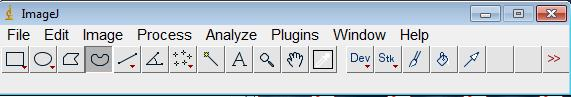
\includegraphics{/images/Figure2.jpg}
\caption{Figure 2}
\end{figure}

\begin{figure}
\centering
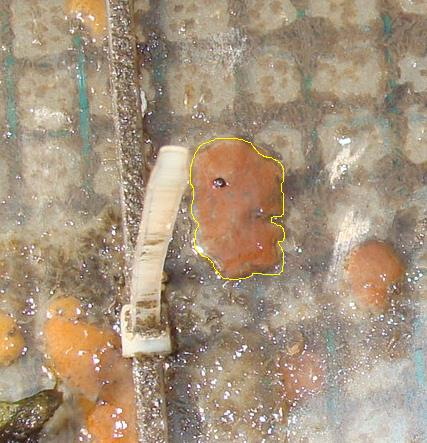
\includegraphics{/images/Figure3.jpg}
\caption{Figure 3}
\end{figure}

\begin{enumerate}
\def\labelenumi{\arabic{enumi}.}
\setcounter{enumi}{4}
\item
  Repeat step 4 with a different colony. Notice that if you didn't close
  the ``Results'' dialog box, your first measurements are still there.
\item
  Repeat until you have measured all species on the panel.
\item
  It's very likely you will have more than one colony of the same
  species, or more than one area value for the same species. Make sure
  to add these up before recording on your spreadsheet for analysis. For
  example, for one colony of \emph{Botrylloides violaceous}, you may
  have an area value of 4.35. For another colony of this species, the
  area is 1.53. Therefore, the total area is 5.88.
\end{enumerate}

\subsection{Recording data in a
spreadsheet}\label{recording-data-in-a-spreadsheet}

Record your data in a spreadsheet. You will want to include Date, Panel
number and identification, side, depth, species, and area for variables.
Figure 4 below shows a suggested format for data entry. (DMC = Darling
Marine Center)

\begin{figure}
\centering
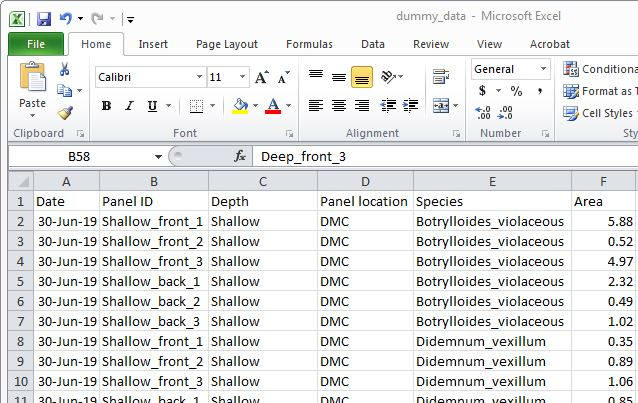
\includegraphics{/images/Figure4.jpg}
\caption{Figure 4}
\end{figure}

\subsection{Visualizing data}\label{visualizing-data}

\begin{enumerate}
\def\labelenumi{\arabic{enumi}.}
\tightlist
\item
  Be sure to save your
\end{enumerate}

\subsection{Statistical analysis}\label{statistical-analysis}

\subsection{Option 2: using a grid to count frequency of
organisms}\label{Option2}

Pros: Faster processing. Cons: With a sparsely populated panel, some
species may be missed.


\end{document}
